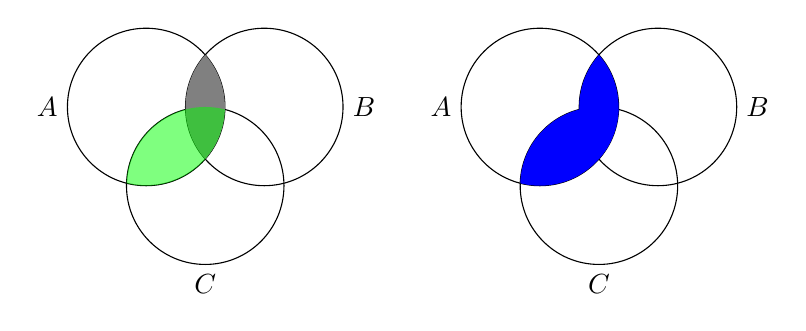
\begin{tikzpicture}
\begin{scope}
\def\firstcircle{(0,0) circle (1)}
\def\secondcircle{(1.5,0) circle (1)}
\def\thirdcircle{(0.75,-1) circle (1)}

\node at (-1,0) [left] {$A$};
\node at (2.5,0) [right] {$B$};
\node at (0.75,-2) [below] {$C$};

\draw \firstcircle;
\draw \secondcircle;
\draw \thirdcircle;

\begin{scope}
\clip \firstcircle;
\clip \secondcircle;
\fill[gray] \secondcircle;
\end{scope}
\begin{scope}
\clip \firstcircle;
\clip \thirdcircle;
\fill[semitransparent,green] \thirdcircle;
\end{scope}
\end{scope}

\node at (3.25,-0.75) {\Large \Ra};

\begin{scope}
\def\firstcircle{(5,0) circle (1)}
\def\secondcircle{(6.5,0) circle (1)}
\def\thirdcircle{(5.75,-1) circle (1)}

\node at (4,0) [left] {$A$};
\node at (7.5,0) [right] {$B$};
\node at (5.75,-2) [below] {$C$};

\draw \firstcircle;
\draw \secondcircle;
\draw \thirdcircle;

\begin{scope}
\clip \firstcircle;
\clip \secondcircle;
\fill[blue] \secondcircle;
\end{scope}
\begin{scope}
\clip \firstcircle;
\clip \thirdcircle;
\fill[blue] \thirdcircle;
\end{scope}
\end{scope}
\end{tikzpicture}
